\begin{frame}
  \frametitle{Linear Models}
  \begin{multicols}{2}
    Objective: minimize error over all training data wrt their labels\\
    $ F(\boldsymbol{X}) = \beta_{0} +  \sum_{j=1}^{p} x_{j} \beta_{j} $\\  
    Smoothing model using regularization by varying $\lambda$\\
    $ F(\boldsymbol{X}) = \beta_{0} +  \sum_{j=1}^{p} x_{j} \beta_{j} + \lambda \sum_{j=1}^{p} \beta_{j}^2 $
  \end{multicols}
  \begin{figure}[h!]
    \begin{minipage}{0.5\textwidth}
      \centering
      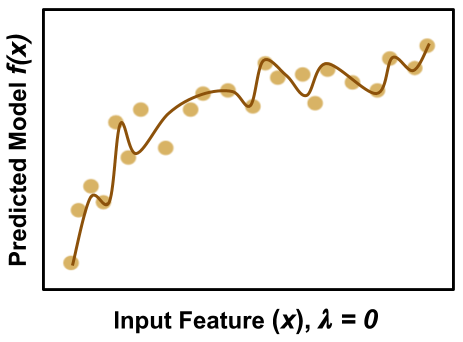
\includegraphics[width=0.85\linewidth]{./figures/regularization_n.png}
    \end{minipage}%
    \begin{minipage}{0.5\textwidth}
      \centering
      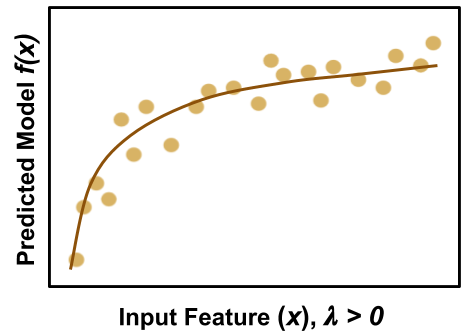
\includegraphics[width=0.85\linewidth]{./figures/regularization_y.png}
    \end{minipage}
    \caption{How regularization might affect the generalizability of an ML model}
  \end{figure}
\end{frame}

\begin{frame}
  \frametitle{Nearest Neighbor Methods}
  \begin{minipage}{0.4\textwidth}
    Objective: minimum distance between test sample and training instance(s)
    $$ Y(\boldsymbol{X}) = \frac{1}{k} \sum_{x_i \in N_k(\boldsymbol{X})} y_i $$
  \end{minipage}%
  \begin{minipage}{0.6\textwidth}
    \begin{figure}[h!]
      \centering
      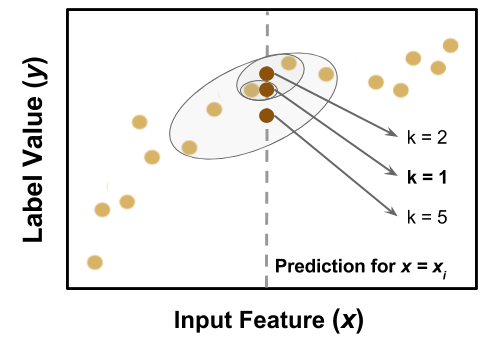
\includegraphics[height=0.5\textheight]{./figures/nn-fig.png}
      \caption{Illustration of the regularization effects by choosing \textit{k}}
    \end{figure}
  \end{minipage}
\end{frame}

\begin{frame}
  \frametitle{Support Vector Machines and Regression}
  \begin{figure}
    \centering
    \begin{minipage}{0.5\textwidth}
      \centering
      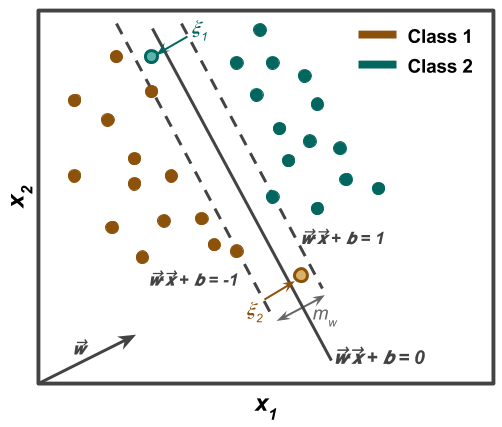
\includegraphics[width=\linewidth]{./figures/svm.png}
    \end{minipage}%
    \begin{minipage}{0.5\textwidth}
      \centering
      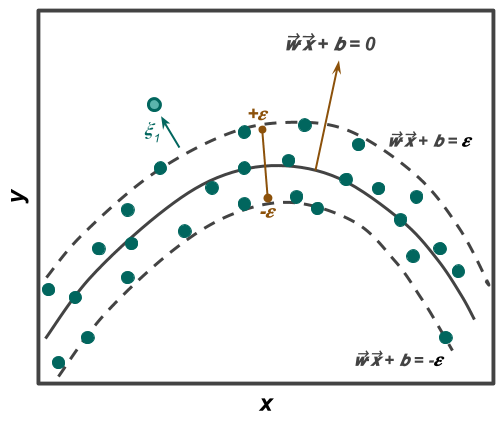
\includegraphics[width=\linewidth]{./figures/svr-a.png}
    \end{minipage}
    \caption{Classification with SVM and regression with SVR}
  \end{figure}
\end{frame}

\begin{frame}
  \frametitle{Support Vector Regression with Many Dimensions}
  \begin{minipage}{.5\textwidth}
    Objective: minimize margin width and outliers
    \scriptsize
    \begin{equation*}
      \begin{split}
        min\ & \frac{1}{2} \lVert w \rVert ^{2} + C \sum_{i} \xi_{i} \\
        subject\ to:\ \ & \lvert y_i - (w \phi(x_i) + b) \rvert \leq \varepsilon + \xi_i \\
        where:\ & w = \sum_{i} \alpha_i y_i \phi(x_i) \\
        and:\ & K(x_i, x_j) = \phi(x_i) \phi(x_j) = e^{\gamma \lVert x_i - x_j \rVert ^{2}}
      \end{split}
    \end{equation*} 
    \normalsize
  \end{minipage}%
  \begin{minipage}{.5\textwidth}
    \centering
    \begin{figure}
      \centering
      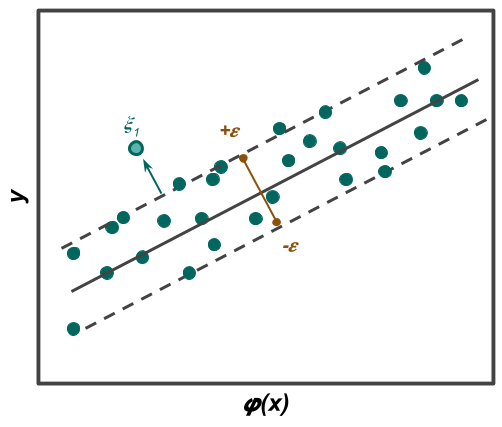
\includegraphics[width=\linewidth]{./figures/svr-b.png}
      \caption{Diagram showing the use of the kernel trick with SVR}
    \end{figure}
  \end{minipage}
\end{frame}

\begin{frame}
  \frametitle{Model Smoothing}
  \begin{enumerate}
    \item Regularization (reduce weights of features)
    \item Dimensionality Reduction (delete features)
    \begin{itemize}
      \item \makebox[3.25cm]{Manual\hfill : \                } some metric
      \item \makebox[3.25cm]{Manual\hfill : \                } domain knowledge
      \item \makebox[3.25cm]{Manual \& Statistical\hfill : \ } factor analysis
      \item \makebox[3.25cm]{Statistical\hfill : \           } principal components analysis (PCA)
      \item \makebox[3.25cm]{Statistical\hfill : \           } independent components analysis (ICA)
    \end{itemize}
  \end{enumerate}
\end{frame}
